\section{Introduction}\label{sec:introduction}
%------------------------- Introduction -------------------------
Artificial Intelligence (AI) and Machine Learning (ML) methods have many areas of applications. It allows us to automate manual processes, make sense of complex data, and learn patterns not readily available to humans. Today, the use of ML methods can be found in most industries, such as fraud detection, diagnosing disease, and increase efficiency in manufacturing processes \cite{forbes:2023:machine_learning}. As AI and ML models are becoming more advanced, they require more data, and the energy consumption of training them increase. However, these resources can could also impact the environment in a negative manner, and it is important to think of the complexity of a model compared to the complexity of the problem. Complex is not always better! 

In this project I will focus on Linear Regression, and study the effect on model perfomance when Ridge and Lasso regularization is included. In addition, I will compare the predictive performance on synthetic data from the Franke function, with more complex data of real terrain. To analyse the models in more detail, I will use resampling methods such as bootstrap and cross-validation, and study the bias-variance trade-off when increasing feature complexity.

In Section II, I will present the methods and tools used in this project. Continuing with Section III, where I show the results and discuss my findings. In Section IV, I conclude and discuss possible future work.


\section{Methods}\label{sec:methods}
%------------------------- Theory -------------------------------
Linear regression is a easy method to fit a line to a set of data points, and the goal is to reduce the total error of the fit. The measure of error to avoid negative sums and calculating absolute sums, we use the sum of squared residuals to evaluate the fit of the line. To find the optimal fit of the line, we calculate the derivative of least squared error and find where it is equal to zero.

Regularization techniques, such as Ridge and Lasso regression, is a way to counteract overfitting. It introduces some bias to reduce the variance, by adding a penalty to the slope where lambda determines how much penalty, or bias, is added. Lambda equal zero gives us OLS. The effect of adding this penalty, when increasing lambda the prediction becomes less sensitive to the input. ridge regression can be used to fit data when you don't have enough data points to fit the number of features. Inversion of matrices with null-values, singular design matrices. To find beta we need to find the inverse of XTX, which is not always possible.

%------------------------- Data ---------------------------------
\subsection{Data}\label{ssec:data}
To implement the regression methods, I used synthetic data generated from the two-dimensional Franke function \eqref{eq:franke_function}, commonly used as a test function in polynomial fitting. The function was used to generate data, which was used to train and test the models. 
\begin{equation}\label{eq:franke_function}
\begin{split}
    f(x, y) &= \frac{3}{4} \exp(- \frac{(9x-2)^{2}}{4} - \frac{(9y-2)^{2}}{4} ) \\
    &+ \frac{3}{4} \exp(- \frac{(9x-2)^{2}}{4} - \frac{(9y-2)^{2}}{4} ) \\
    &+ \frac{3}{4} \exp(- \frac{(9x+1)^{2}}{49} - \frac{(9y+1)}{10} ) \\ 
    &- \frac{1}{5} \exp(- (9x-4)^{2} - (9y-7)^{2} ) 
\end{split}, 
\end{equation}
where $x, y \in [0, 1]$. I generated data points from a uniform distribution, to ensure a good representation of the domain. The data was not scaled as the input to the function was scaled, resulting in the output being scaled to that domain.

In addition to synthetic data, I tested the models on real terrain data. The real data was generated using the EarthExplorer \cite{usgov:2024:earthexplorer}, with selected World Features. To study the performance of the models on various terrain, I generated data set which included different features. Information on the terrain data can be found in Table \ref{tab:terrain_data}, in Appendix \ref{ap:terrain_data}.

The terrain data was not preprocessed, which required it to be scaled. I started with standard scaling, and also tested min-max scaling. However, these did not work for only scaling the terrain data values, I standardized the terrain data by subtracting the mean value, and dividing by the standard deviation.

Both the function data and the terrain data was split up in train and test set.


%------------ Linear regression ------------------------------
\subsection{Regression methods}\label{ssec:regression_methods}
For problems of a continuous nature, linear regression methods are commonly used, as they provide analytical expressions which can provide statistical insight. The aim of regression methods is to find a function which describes the data, by minimizing the difference from observed to predicted data. That is, given a set of data $\mathbf{y}$, the aim is to find a continuous function $f$ which model the data as
\begin{equation*}
    \mathbf{y} = f( \mathbf{x} ) + \mathbf{\epsilon}, 
\end{equation*}
where $\mathbf{\epsilon} \in \mathcal{N}(0, \sigma^{2})$. In this project I will apply Ordinary Least Squares regression to find an approximation of the data 
\begin{equation*}
    \mathbf{\Tilde{y}} = \mathbf{X} \mathbf{\beta},
\end{equation*}
where $\mathbf{\beta}$ are the optimal parameters. More specifically, I want to find the relationship between the input features and the target, by determining the coefficients. 

To measure the quality of the model, the loss function is defined as the Mean Squared Error
\begin{equation}\label{eq:mse}
    C (\mathbf{\beta}) = \frac{1}{n} \big( (\mathbf{y} - \mathbf{X} \mathbf{\beta})^{T} (\mathbf{y} - \mathbf{X} \mathbf{\beta}) \big).
\end{equation}

To find the optimal values $\mathbf{\beta}$, I solve the derivative of the loss function $\frac{\partial C (\beta)}{\partial \beta} = 0$ which minimizes the spread of \eqref{eq:mse}. This can be written as  
\begin{equation}
    \mathbf{\beta} = (\mathbf{X}^{T}\mathbf{X})^{-1} \mathbf{X}^{T} \mathbf{y},
\end{equation}
given that the matrix $\mathbf{X}^{T}\mathbf{X}$ is invertible.


%------------ Regularization ------------------------------
Ridge and Lasso regression include a regularixation term, which can fix the issue when the features are linearly dependent. The term is controlled by a hyperparameter $\lambda$, and penalise the loss function. For Ridge regression the optimal parameters are
\begin{equation}\label{eq:ridge_beta}
    \mathbf{\beta} = (\mathbf{X}^{T}\mathbf{X} + \lambda \mathbf{I})^{-1} \mathbf{X}^{T} \mathbf{y},
\end{equation}
where $\mathbf{I}$ is the identity matrix. The loss function to optimize can be written as
\begin{equation}\label{eq:ridge_cost}
    C (\mathbf{\beta}) = \frac{1}{n} || \mathbf{y} - \mathbf{X} \mathbf{\beta} ||_{2}^{2} + \lambda || \mathbf{\beta} ||_{2}^{2} ,
\end{equation}
where $|| \mathbf{\beta} ||_{2}^{2}$ is the norm-2.

For Lasso regression we find the optimal parameters $\mathbf{\beta}$ by minimizing
\begin{equation}\label{eq:lasso_cost}
    C (\mathbf{\beta}) = \frac{1}{n} || \mathbf{y} - \mathbf{X} \mathbf{\beta} ||_{2}^{2} + \lambda || \mathbf{\beta} ||_{1} ,
\end{equation}
where $|| \mathbf{\beta} ||_{1}$ is the norm-1. This result in a discontinuous derivative of the loss function, which does not give a direct analytical expression as with OLS and Ridge. To solve this I have used scikit-learn's implementation of Lasso.


%------------ Model evaluation --------------------------------
To evaluate the performance of the model, I calculate the mean squared error (MSE) and the R2-score, . The MSE measures the average squared difference between the predicted value and the true value, which makes it sensitive to larger differences. 
\begin{equation}\label{eq:mse}
    MSE(\mathbf{y}, \mathbf{\Tilde{y}}) = \frac{1}{n} \sum_{i=0}^{n-1} (y_{i} - \Tilde{y}_{i})^{2}.
\end{equation}

The R$^{2}$-score indicate the accuracy of the model prediction, where a score of $1$ is a perfect fit.
\begin{equation}\label{eq:r2}
    R^{2}(\mathbf{y}, \mathbf{\Tilde{y}}) = 1 - \frac{\sum_{i=0}^{n-1} (y_{i} - \Tilde{y}_{i})^{2}}{\sum_{i=0}^{n-1} (\Tilde{y}_{i} - y_{i})^{2}}.
\end{equation}

as well study the bias-variance trade-off. 


\section{Results}\label{sec:results}
%------------ Part a ------------------------------------------
Scaling... 
I generated data from the franke function, both with and without stochastic noise, and performed an OLS regression analysis up to polynomial of degree 5. The feature data was not scaled, as both input features were sampled from a uniform distribution $\in [0, 1]$, resulting in the function data being scaled to that domain. Before training the model, the input and target data was split into train and test set, where the test set contained $20\%$ of the original data.

I computed the MSE and R$^{2}$-score for predictions on both data set, the result is shown in Figure \ref{fig:ols_error} and Figure \ref{fig:ols_error_noisy}, respectively.

\begin{figure}
    \centering
    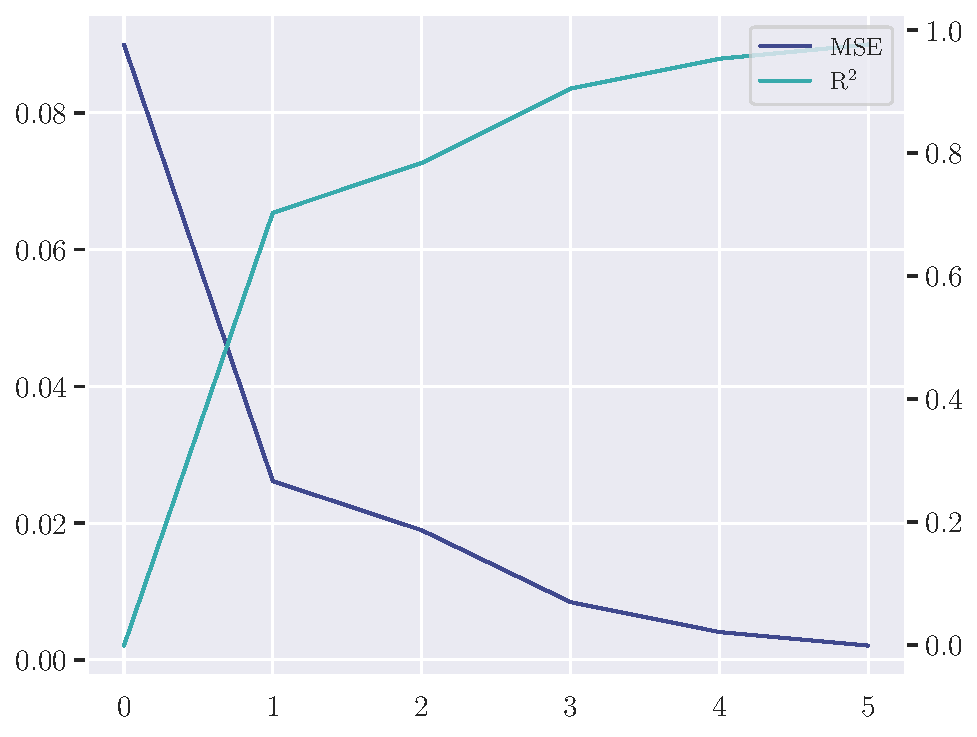
\includegraphics[width=0.9\linewidth]{project-1/latex/figures/ols_error.pdf}
    \caption{MSE and R$^{2}$-score computed on test data, as a function of the polynomial degree of the input features. The function data was generated without stochastic noise.}
    \label{fig:ols_error}
\end{figure}

\begin{figure}
    \centering
    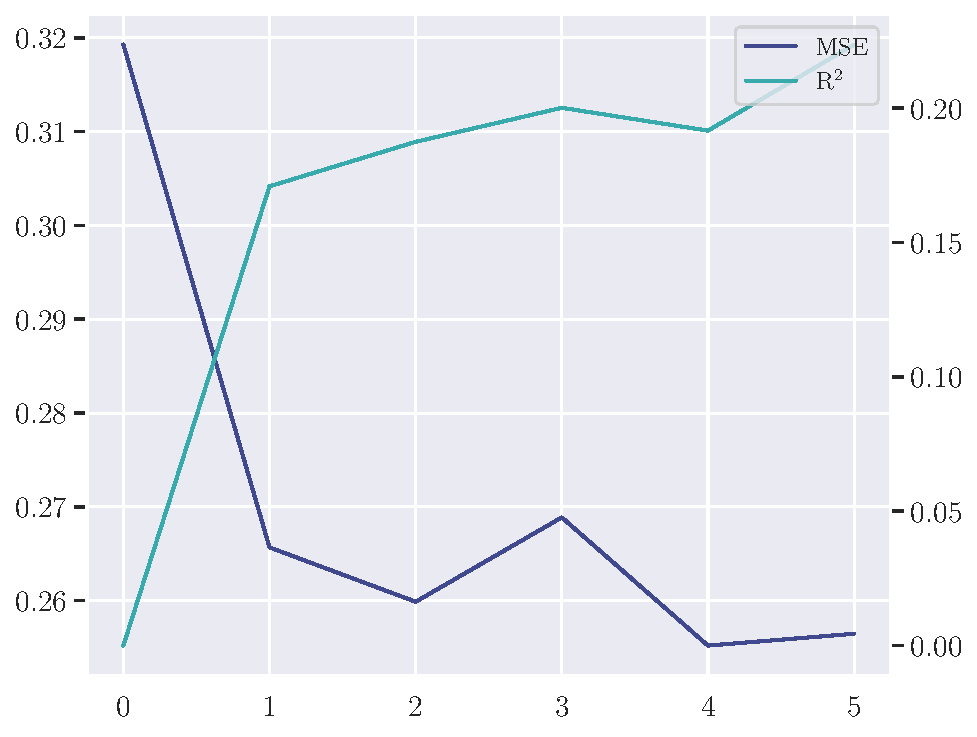
\includegraphics[width=0.9\linewidth]{project-1/latex/figures/ols_error_noisy.pdf}
    \caption{MSE and R$^{2}$-score computed on test data, as a function of the polynomial degree of the input features. The function data includes stochastic noise $\epsilon \in \mathcal{N}(0, 1)$.}
    \label{fig:ols_error_noisy}
\end{figure}

When noise is included in the function data, the error increases for all polynomial degrees. Since the R$^{2}$-score determines how large a proportion of the variance in the dependent variable is explained by the independent variable, it seems the model only explains the input features.

Looking at $\beta$-values for the model fitting the function data without noise in Figure \ref{fig:ols_beta}, and the function data with noise Figure \ref{fig:ols_beta_noisy}. As the polynomial degree increase, the absolute values of $\beta$ increase. However, both the absolute values and variance between each $\beta_{i}$ increase when noise is included in the function.  
\begin{figure}
    \centering
    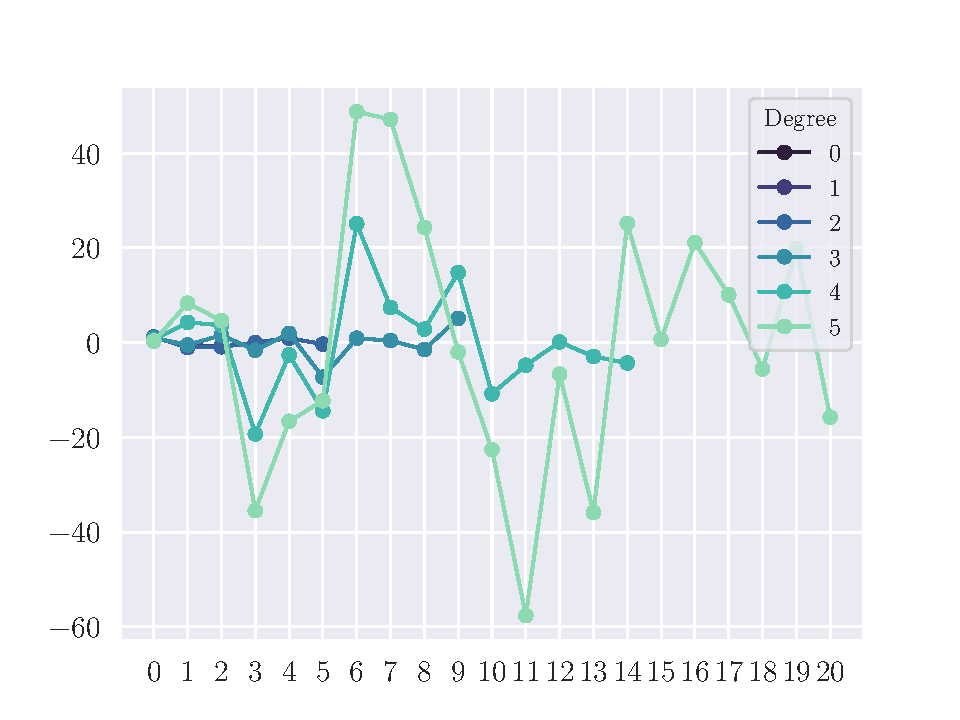
\includegraphics[width=0.9\linewidth]{project-1/latex/figures/ols_beta.pdf}
    \caption{The figure shows beta values for different polynomial degree.}
    \label{fig:ols_beta}
\end{figure}

\begin{figure}
    \centering
    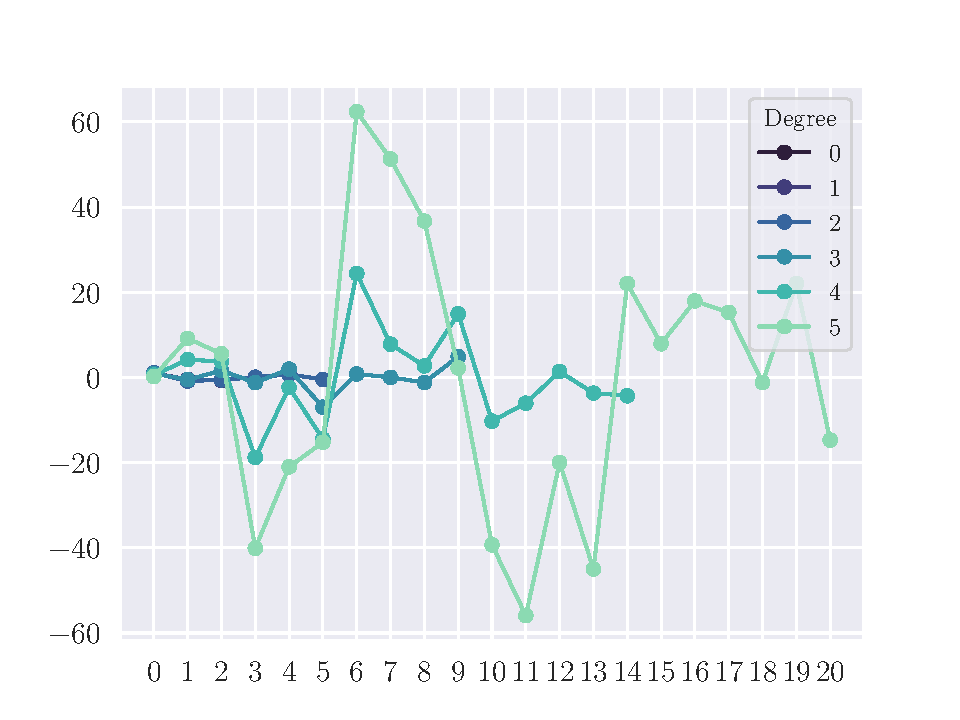
\includegraphics[width=0.9\linewidth]{project-1/latex/figures/ols_beta_noisy.pdf}
    \caption{The figure shows beta values for different polynomial degree, when the function includes noise.}
    \label{fig:ols_beta_noisy}
\end{figure}

I continued the regression analysis with data from the Franke function which included noise.

%------------ Part b ------------------------------------------
To determine a range for the optimal values of $\lambda$, I trained and tested the Ridge model on $100$ values, where Log$_{10}(\lambda) \in [-10, 10]$. The result can be found in Figure \ref{fig:test_lmbda_range}, in Appendix \ref{ap:additional_analysis}. However, it indicated that negative values of were likely to be better for further analysis. I continued with $100$ values, where Log$_{10}(\lambda) \in [-15, 5]$, the result is found in Figure \ref{fig:lmbda_opt}.

\begin{figure}
    \centering
    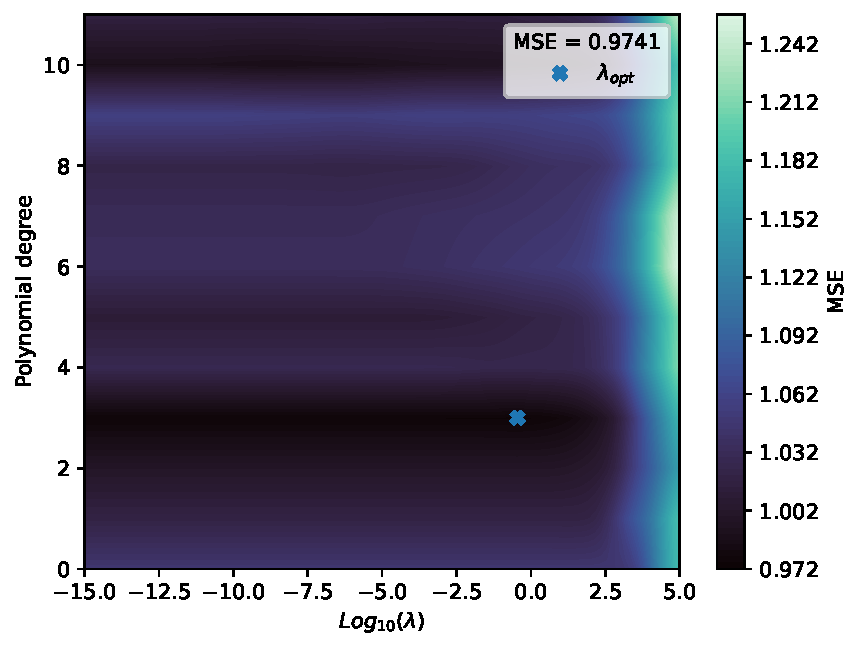
\includegraphics[width=0.9\linewidth]{project-1/latex/figures/lmbda_opt.pdf}
    \caption{The figure shows MSE as a function of $\lambda$ and polynomial degree $P$, where the optimal value for $\lambda$ and $P$ is marked by an X.}
    \label{fig:lmbda_opt}
\end{figure}


%------------ Part c ------------------------------------------




%------------ Part d ------------------------------------------




%------------ Part e ------------------------------------------




%------------ Part f ------------------------------------------




%------------ Part g ------------------------------------------



